% Final presentation for EECS 441 at Northwestern University
% Given on 6.7.12 by Maciej Swiech and Marcel Flores

\documentclass{beamer}
\usetheme{Madrid}
\usepackage{graphicx}
\usepackage{listings}

\begin{document}
\title{Hardware Transactional Memory without the Hardware}
\author{Zach Bischof, Marcel Flores, Maciej Swiech}
\institute{Northwestern University}
\date{\today}

\begin{frame}[plain]
  \titlepage
\end{frame}

\section{Transactions}
\frame{\frametitle{Table of Contents}\tableofcontents}

\begin{frame}{Transactions}
  Transactions are taken from the world of databases, where units of work are
  performed in isolation from the system, and can be aborted so that from the
  point of the view of the rest of the system, it looks like no changes ever
  happened.

  A database transaction must be:
  \begin{itemize}
    \item Atomic
    \item Consistent
    \item Isolated
    \item Durable
  \end{itemize}
\end{frame}

\section{Why Transactions?}
\begin{frame}{Why Transactions?}
  \begin{itemize}
    \item Locks are complicated, expensive, and ... \pause pessimistic
    \pause
    \item Transactions are optimistic - very few (if any) memory locations in a locked 
    region actually get altered by other processess, so locking them becomes
    an overhead that need not be paid.
    \pause
    \item Locks require a thread to wait for an entire region to be released, which
    does not scale well in increasingly parallel programming design.
    \pause
    \item Transactions allow actions to go on until they necessarily would interfere
    or be interfered with, with a abort handler scenario.
  \end{itemize}

\end{frame}
  
\begin{frame}{Why Transactions?}
  So by using transactions we are afforded:
  \begin{itemize}
    \item Cheap critical sections of code
    \pause
    \item Freedom from having to manage tons of locks
    \pause
    \item Code that can operate as if no other threads were running
  \end{itemize}
\end{frame}

\section{Intel Implementation}
\begin{frame}{Intel Implementation}
  \begin{definition}
  A \textbf{transaction} is a sequence of memory operations that are 
  performed by a process such that, to all other processes, the operations 
  seem to have been performed atomically. Furthermore, the operations must 
  appear to the process performing the transaction as having happened one
  after another, with no interference from other processes
  \end{definition}
\end{frame}

\begin{frame}{Intel Implementation (Haswell)}
  \begin{block}{XBEGIN rel32}
  Starts off a transactional block, specifying a relative location to jump to
  in the case of an XABORT
  \end{block}

  \pause

  \begin{block}{XABORT imm8}
  Aborts a transaction, placing the code in EAX and ignoring all changes made
  during the transaction
  \end{block}

  \pause

  \begin{block}{XEND}
  Ends a transational block, committing all changes made during the
  transaction
  \end{block}
\end{frame}

\section{Palacios Implementation}
\begin{frame}{Palacios Implementation}
  \begin{center}
    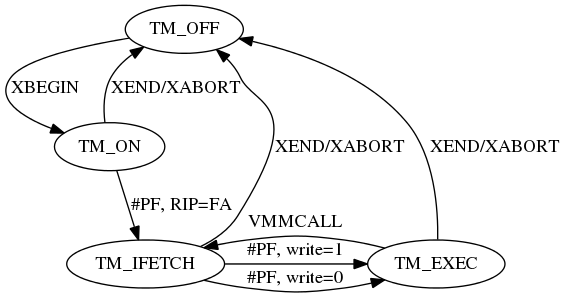
\includegraphics[width=3.0in]{fsm.png}
  \end{center}
    
  The finite state machine we use in our implementation of Transactional
  Memory
\end{frame}

% xbegin, mem read/write, vmcall injection, xend
\begin{frame}{XBEGIN}
  When the Host OS sees an XBEGIN, it throws an Undefined Opcode Exception,
  which we catch. We now enter the TM\_ON portion of our FSM, and set up the
  following:

  \begin{itemize}
    \item Allocate necessary data structures to keep track of Guest OS state
    \item Blast away the VTLB
  \end{itemize}
\end{frame}
    
\begin{frame}{IFETCH}
  We come into the VMM having seen an ifetch Page Fault, and let the VTLB do its
  thing

  \begin{itemize}
    \item Store the next instruction and replace it with a hypercall
  \end{itemize}
\end{frame}

\begin{frame}{Data Operations}
  The next Page Fault we receive is a read or write, we need to handle it
  accordingly

  \begin{itemize}
    \item Check The TLB error flag to see if read or write
    \item Record it in the appropriate data structures
  \end{itemize}
\end{frame}

\begin{frame}{hypercall}
  When we see our hypercall, we know that the 'current' instruction has finished,
  we need to clean up and restore the next instruction

  \begin{itemize}
    \item Restore the stored next instruction
    \item Blast away the VTLB
    \item The cycle starts over
  \end{itemize}
\end{frame}

\begin{frame}{Abort}
  Either the code or a condition has signalled an abort

  \begin{itemize}
    \item Turn off TM state
    \item Restore the next instruction
    \item Free all of our data structures
    \item Change RIP to point to abort handler
  \end{itemize}
\end{frame}

\begin{frame}{XEND}
  The transactional block has come to a successful end, we need to commit the
  changes

  \begin{itemize}
    \item Turn off TM state
    \item Go through our data structures, copying entries into memory
    \item Free all of our data structures
  \end{itemize}
\end{frame}

\section{Assumptions}
\begin{frame}{Current Assumptions}
  \begin{itemize}
    \item Instructions in transaction can be decoded
    \item Entire transaction will fit on a page
    \item All instructions occur on the same page
    \item Interrupts can be ignored
    \item Single core environment
  \end{itemize}
\end{frame}

\section{Future Work}
\begin{frame}{Future Work}
  \begin{itemize}
    \item Fix all assumptions
    \item Add Multicore Support
    \item Add Intel Support (?)
    \pause
    \item Optimizations...
  \end{itemize}
\end{frame}

%\begin{frame}[fragile]{Test Code}
  %\tiny
  %\begin{lstlisting}{language=c}
  %int main(){
      %long x = 0;
      %long y = 2;
      %printf("%ld %ld\n",x, y);  
      %asm("movq $1, %%rax;"
          %"test: xbegin fail;"
          %"addq (%1), %%rax; "
          %"xend; "
          %"jmp success;"
          %"fail:;"
          %"ret; "
          %"success:; "
          %"movq %%rax, %0"
          %: "=r"(y)
          %: "r"(&x)
          %: "%rax"
         %);
      %printf("%ld %ld\n",x, y);  

      %return 0;
  %}
  %\end{lstlisting}
%\end{frame}
\end{document}
